% mycsrf 'for beeing included' snippet template
%
% (c) Karsten Reincke, Frankfurt a.M. 2012, ff.
%
% This text is licensed under the Creative Commons Attribution 3.0 Germany
% License (http://creativecommons.org/licenses/by/3.0/de/): Feel free to share
% (to copy, distribute and transmit) or to remix (to adapt) it, if you respect
% how you must attribute the work in the manner specified by the author(s):
% \newline
% In an internet based reuse please link the reused parts to mycsrf.fodina.de
% and mention the original author Karsten Reincke in a suitable manner. In a
% paper-like reuse please insert a short hint to mycsrf.fodina.de and to the
% original author, Karsten Reincke, into your preface. For normal quotations
% please use the scientific standard to cite
%


%% use all entries of the bibliography

\subsection{EasyABC ($\bigstar\bigstar\bigstar\bigstar$)}

\parpic(2.5cm,1cm)[r][t]{
\includegraphics[width=2.5cm]{logos/easyabc-300dpi.png}}
\label{EasyABC}Seine Repositoryseite sagt von \acc{EasyABC}, es sei in Python
geschriebenes Notensatzprogramm, das für die graphische Darstellung auf das
Kompatibilitätsframework \acc{WxWidgets}
zurückgreife.\footnote{\cite[vgl.][\nopage wp]{EasyAbc2017a}. Die zu startende
Datei \texttt{easyabc.py} lizenziert das Programm im Header unter der GPL-3.0.
Damit ist es freie Software.} Die letzte Version stammt vom Mai
2018.\footcite[vgl.][\nopage wp]{EasyAbc2017c} Das Open Source Projekt pflegt
außerdem eine Projekthomepage, die Installationsoptionen
auflistet.\footcite[vgl.][\nopage wp]{EasyAbc2017b} Neben diesen beiden
Anlaufpunkten existiert noch die (veraltete) Homepage des ursprünglichen
Programmierers.\footcite[vgl.][\nopage wp]{Liberg2015a} Vom Typ her gehört
\acc{EasyABC} zu den semi-graphischen Editoren.

(Aktuelle) Distributionen werden \acc{EasyABC} eher nicht mit
anbieten.\footnote{Ubuntu 18.04 jedenfalls offeriert kein entsprechendes Paket.}
Denn -- laut \acc{EasyABC} Installationsanleitung -- gäbe es intendiert keine
entsprechenden Installations- oder Binärpakete: \acc{EasyABC} solle per Shell --
über den Befehl \texttt{python easy\_abc.py} -- direkt aus dem heruntergeladenen
Ordner mit den Softwarequellen gestartet werden, damit das Programm all seine
Resourcen finde.\footnote{Das Quellpaket enthält eine Linuxanleitung
(\texttt{using\_EasyABC\_in\_Windows.txt}) und eine Windowsanleitung
(\texttt{using\_EasyABC\_in\_Linux.txt}), die jeweils auflisten welche
Zusatzpakete installiert sein müssen, bevor man \acc{EasyABC} erfolgreich
starten kann. Ubuntu 18.04 Nutzer müssen bei der Abarbeitung der Liste
aufpassen: Python3 ist Distributionsstandard, während Python2.7 nur 'nebenbei'
angeboten wird. Die letzte Version von \acc{EasyABC} verlangt aber noch
Python2.7 und das dazu passende wx-Paket. Deshalb gilt es bei Ubuntu 18.04, die
Python3-Module so weit als möglich zu deinstallieren, bis der Befehl
\texttt{python --version} eine 2.7-Version ausgibt. Danach reicht es, das
Kommando \texttt{sudo apt-get install python-wxgtk-media3.0}
abzusetzen. Anschließend kann man \acc{EasyABC} erfolgreich starten.}

Nach dem Start bietet sich dem 'Notenschreiber' ein viergeteiltes Fenster an: Im
unteren rechten Bereich notiert der Komponist, Arrangeur oder
Musikwissenschaftler seine Noten im \acc{ABC}-Format. Im oberen rechten Bereich
wird daraus -- on the fly -- der entsprechende Notentext abgeleitet und
angezeigt. Der obere linke Teil des Fensters listet die offenen 'Songs' auf. Und
der untere linke Fensterteil enthält den Clou des Ganzen: einen -- auf die
Cursorposition im Notentext bezogenen -- kontextsensitiven 'Next-Steps'-Bereich,
in dem -- direkt per Klick ausführbar -- aufgelistet wird, was an der fraglichen
Stelle wie modifiziert werden kann. Für unsere Referenzkadenz II, die
\acc{EasyABC} in den Grenzen des Backens erfolgreich darstellen kann, sähe das
so aus:

\begin{center}
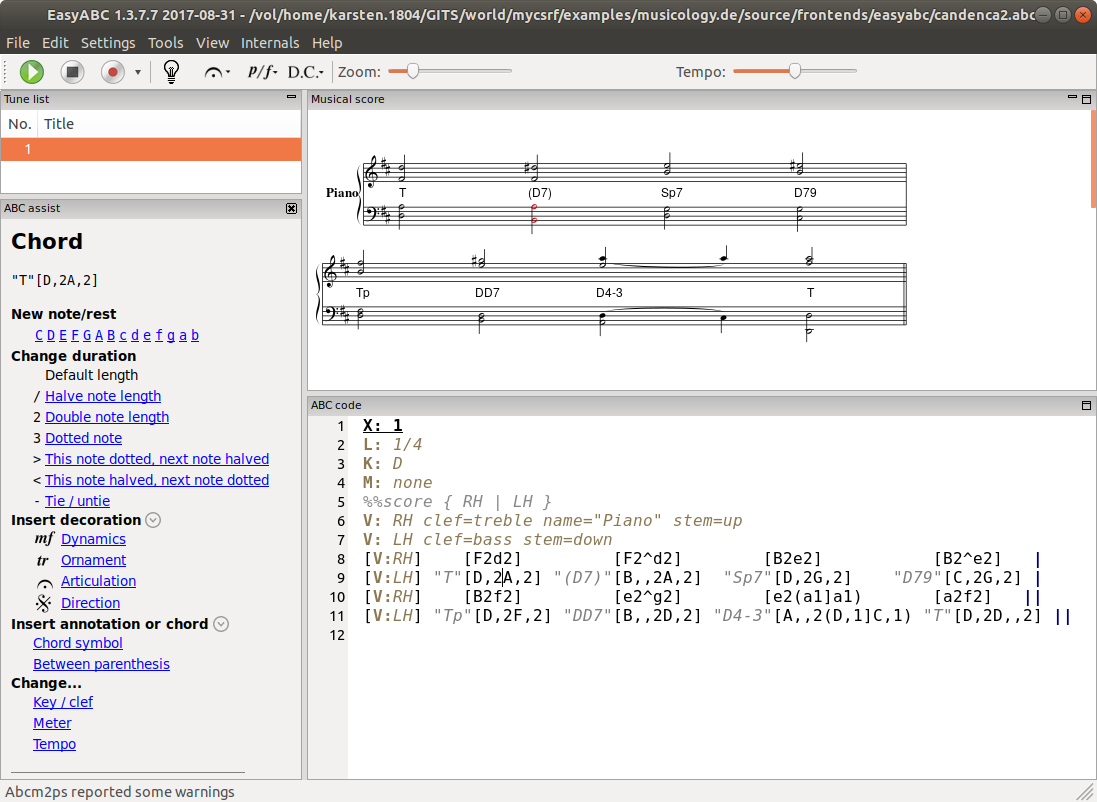
\includegraphics[width=0.9\textwidth]{frontends/easyabc/easyabc-cadenca2-300dpi.png}
\end{center}

Beim kontextsensitiven Editieren setzt man den Cursor im rechten unteren
Editorfeld in einen 'Akkord' bzw. auf eine 'Note' -- in unserem Beispiel Zeile
9, \texttt{[D,2A,2]} --, den oder die das System in der rechten oberen
Visualisierung rot einfärbt. Dieser per Cursor ausgewählte Bereich wird im
linken unteren Fensterteil analysiert und beschrieben, bevor darunter all die
Modifikationen und Erweiterungen aufgelistet werden, die an dieser Stelle in
diesem Kontext von der \acc{ABC}-Syntax her möglich sind. \acc{EasyABC} bietet
damit eine zukunftsweisende und trickreiche 'Code-Completion' an, die die
Tipparbeit wirklich zu vereinfach vermag.

Schließlich bliebe zu erwähnen, dass man das, was man im Editorfenster
eingegeben hat, als \acc{ABC}-Code speichern oder als PDF-, MIDI, MusicXML- oder
HTML-Datei exportieren kann. Außerdem bietet \acc{EasyABC} bei gelungener
MIDI-Integration die Möglichkeit, das Eingegebene auch zu hören.

In Verbindung mit den Konvertern bietet \acc{EasyABC} den Musikwissenschaftlern
als textbasierter Editor mit automatisierter Visualisierung also ein sehr gut zu
nutzendes Frontend für die \acc{ABC}-Notationsmethode.

% this is only inserted to eject fault messages in texlipse
%\bibliography{../bib/literature}
